\documentclass[11pt]{article}
\usepackage{amsmath, amssymb}
\usepackage{geometry}
\usepackage{hyperref}
\usepackage{graphicx}
\usepackage{booktabs}
\geometry{margin=2.5cm}
\emergencystretch=2em

\newcommand{\ket}[1]{|#1\rangle}
\newcommand{\bra}[1]{\langle#1|}
\newcommand{\Oedge}{X_0 Z_1\cdots Z_{L-2} X_{L-1}}
\newcommand{\Tr}{\operatorname{Tr}}

\title{Block 4 Notes: Noise on the Edge-String Diagnostic}
\author{}
\date{\today}

\begin{document}
\maketitle

\section{Purpose}

Weeks 6 and 7 established the edge-string observable
\[
  O_{\mathrm{edge}} = \Oedge
\]
as the phase diagnostic. Week 6 validated the observable with exact diagonalization (ED), and Week 7 showed that a parity-constrained VQE sweep can reproduce the same curve well enough to serve as a noiseless reference.

Block 4 asks what survives once the circuit is no longer ideal. The broad theory includes state-preparation errors, gate depolarization, readout assignment errors, shot noise, relaxation, dephasing, and optimizer instability. The current code implements only the first controlled slice of that program: a frozen-state edge-string noise test in \texttt{src/block4.py}.

The implemented test freezes state preparation and studies how the validated edge-string signal is degraded by
\begin{itemize}
  \item symmetric readout error with probability $\epsilon$ per measured qubit;
  \item local two-qubit depolarizing noise with probability $p_{2q}$ on nearest-neighbor pairs;
  \item finite-shot sampling with $N_{\mathrm{shots}}=4096$ by default.
\end{itemize}

This separation matters. If we optimized the VQE circuit under noise immediately, a failed curve could come from either physical circuit noise or from the classical optimizer being driven to bad parameters by noisy cost evaluations. The frozen-state test isolates the measurement/noise layer first.


\section{Implemented vs. Not Implemented Yet}

The present code should be understood as a first controlled noise diagnostic, not the full Block 4 noise program.

\subsection*{Implemented in \texttt{block4.py}}
\begin{itemize}
  \item \textbf{Hamiltonian consistency:} uses the same Kitaev/Jordan--Wigner operator, imported through \texttt{qubit\_hamiltonian} from \texttt{block3\_core.py}.
  \item \textbf{Even-parity ED baseline:} the state is obtained with \texttt{ed\_even\_ground\_state}. This is a clean validated baseline, not yet a stored VQE parameter path.
  \item \textbf{Edge-string observable:} imported through \texttt{edge\_string}, so the measured operator is consistent with Blocks 3 and 4.
  \item \textbf{Symmetric readout attenuation:} implemented as the scalar factor $(1-2\epsilon)^L$.
  \item \textbf{Local two-qubit depolarizing noise:} implemented as a density-matrix Pauli channel on nearest-neighbor pairs.
  \item \textbf{Finite-shot sampling:} implemented with binomial sampling through \texttt{shot\_estimate}.
\end{itemize}

\subsection*{Theoretical Context Not Implemented Yet}
\begin{itemize}
  \item \textbf{Explicit measurement-basis gates:} the current code evaluates the edge-string operator directly; it does not build the Hadamard measurement circuit.
  \item \textbf{Asymmetric readout assignment matrix:} there is no $p(1|0)\neq p(0|1)$ model and no additive SPAM-bias term.
  \item \textbf{Amplitude damping / $T_1$ relaxation:} there is no parity-poisoning relaxation channel yet.
  \item \textbf{Phase damping / $T_2$ dephasing:} there is no explicit dephasing channel yet.
  \item \textbf{Noisy VQE optimization:} the optimizer is not run with noisy estimators.
  \item \textbf{Backend-calibrated Qiskit Aer noise model:} the plot uses a simple density-matrix noise model, not hardware calibration data.
\end{itemize}

\section{Source of Truth for the Practical Plot}

The scripted implementation is
\[
  \texttt{src/block4.py}.
\]
It reuses the same project Hamiltonian and operators from \texttt{src/block3\_core.py}. In particular, it imports \texttt{qubit\_hamiltonian}, \texttt{edge\_string}, \texttt{parity}, \texttt{ed\_even\_ground\_state}, and \texttt{shot\_estimate}. The exploratory notebook \texttt{notebooks/Kitaev\_Chain\_Noise\_Simulation.ipynb} is not the source of truth for the Week 8 plot.

For each value of $\mu$, the code constructs the same Jordan--Wigner qubit Hamiltonian used in Block 3,
\[
H(\mu) = -\frac{\mu}{2}\sum_j Z_j
+ \frac{t-\Delta}{2}\sum_j X_jX_{j+1}
+ \frac{t+\Delta}{2}\sum_j Y_jY_{j+1},
\]
then selects the exact even-parity ground state. This gives a clean density matrix
\[
  \rho_0(\mu)=\ket{\psi_+(\mu)}\bra{\psi_+(\mu)}.
\]
The baseline expectation value is
\[
  s_0(\mu)=\Tr\!\left[O_{\mathrm{edge}}\rho_0(\mu)\right].
\]

The present Block 4 plot should therefore be read as a noise test on the validated edge-string baseline, not yet as a full noisy-optimizer VQE result.

\section{What Noise Can Break}

There are two broad failure categories: state preparation and measurement.

\subsection{State Preparation}

In ideal simulation, rotations are exact matrices. On hardware, a rotation is a calibrated pulse. A pulse-amplitude error, timing error, frequency drift, or thermal fluctuation can turn the intended rotation $R(\theta)$ into something closer to $R(\theta+\delta\theta)$. Then the prepared state drifts away from the target ground state.

The edge-string signal is especially sensitive because it is non-local. The Majorana diagnostic depends on the first and last sites being correlated through the chain. In the VQE ansatz this correlation is built through a ladder of entangling operations. Two-qubit gates are usually the noisiest gates in superconducting NISQ hardware, so a gate error can suppress the edge-to-edge correlation even when local observables still look reasonable.

Relaxation can also move the state into the wrong parity sector. In the Jordan--Wigner encoding, qubit occupation tracks fermionic occupation. A $T_1$ event, schematically $\ket{1}\to\ket{0}$, changes occupation and can flip the fermion parity. Since our diagnostic is tied to the even-parity ground-state sector, this kind of parity poisoning is qualitatively more dangerous than simple contrast loss.

These state-preparation mechanisms are theoretical context in the present notes. The current \texttt{block4.py} does not yet simulate pulse errors, $T_1$, $T_2$, or a noisy VQE optimization loop.

\subsection{Measurement}

The edge string is a product of measured eigenvalues. For $L=4$,
\[
  O_{\mathrm{edge}}=X_0Z_1Z_2X_3.
\]
If one measured bit is assigned incorrectly, one factor in the product changes sign, so the whole string result can flip. As $L$ grows, the probability that at least one factor is wrong increases.

Shot noise is different from hardware noise. Even with perfect gates and perfect readout, a finite number of measurements gives a statistical estimator rather than the exact mean. For $N_{\mathrm{shots}}$ shots, a typical scale is
\[
  \sigma \sim \frac{1}{\sqrt{N_{\mathrm{shots}}}}
\]
when the true expectation value is not close to $\pm1$. With the default $N_{\mathrm{shots}}=4096$, this is about $1.6\%$.

The critical regions near $|\mu|\approx2t$ are hardest to classify because the true edge-string signal changes rapidly there. If the physical signal is already small near the transition, readout error, gate noise, and shot noise can make the phase boundary ambiguous.

\section{Frozen Noise Test vs. Noisy Optimization}

There are two distinct experiments:
\begin{enumerate}
  \item \textbf{Frozen-state noise test.} Prepare or assume the validated noiseless state, then apply noise to the state and/or measurement. This asks: if the correct state were available, could the edge-string signal still be read out?
  \item \textbf{Noisy VQE optimization.} Run the variational loop while the cost function is noisy. This asks: can the optimizer find the correct state when every energy estimate is corrupted?
\end{enumerate}

The current \texttt{block4.py} implements the first experiment. It uses the exact even-parity ground state as the clean baseline and then applies controlled noise to that density matrix and expectation value. It does not yet run COBYLA, L-BFGS-B, SPSA, or any optimizer under noisy estimates.

\section{The Pauli-Matrix Helper}

The function \texttt{pauli\_matrix(L, site\_ops)} builds a dense matrix for a Pauli string acting on selected lattice sites. For example,
\begin{verbatim}
pauli_matrix(4, {0: 'X', 1: 'Z', 3: 'Y'})
\end{verbatim}
represents an operator with $X$ on site $0$, $Z$ on site $1$, $Y$ on site $3$, and identity on every unspecified site.

The subtle line is the index reversal:
\[
  \texttt{label[L - 1 - site] = op}.
\]
This is needed because Qiskit writes Pauli labels in big-endian string order, while our physics convention labels the chain sites in little-endian order. Site $0$ is therefore placed at the rightmost character of the Qiskit Pauli string. This matches the convention already used in \texttt{block3\_core.py} for the Hamiltonian, parity, local observables, and edge string.

\section{Readout Error}

For the implemented plot, readout error is symmetric:
\[
  0 \leftrightarrow 1 \quad \text{with probability } \epsilon.
\]
For a single measured Pauli-$Z$ eigenvalue $z=\pm 1$, a symmetric bit flip changes the expectation value by
\[
  \langle z\rangle_{\mathrm{readout}} = (1-2\epsilon)\langle z\rangle_{\mathrm{ideal}}.
\]
The edge string is a product of $L$ measured signs. If the readout errors are independent, the full string is attenuated by
\[
  A_{\mathrm{readout}}(\epsilon,L)=(1-2\epsilon)^L.
\]
This is what \texttt{symmetric\_readout\_scale(epsilon, weight)} returns. In the default plot $L=4$, so
\[
  s_{\mathrm{readout}}(\mu)=(1-2\epsilon)^4s_0(\mu).
\]

\subsection{Broader Theory: Asymmetric Readout and SPAM Bias}

Real readout is often asymmetric. Let
\[
  \alpha=p(1|0),\qquad \beta=p(0|1),
\]
where $\alpha$ is a false-one probability and $\beta$ is a false-zero probability. The single-qubit assignment matrix is
\[
A=\begin{pmatrix}
1-\alpha & \beta\\
\alpha & 1-\beta
\end{pmatrix}.
\]
For a $Z$ measurement vector $(1,-1)^T$, the noisy measurement is
\[
  \langle Z\rangle_{\mathrm{noisy}}
  =(1-\alpha-\beta)\langle Z\rangle_{\mathrm{ideal}}+(\beta-\alpha).
\]
So asymmetric readout does two things: it attenuates the signal and adds a systematic offset. For a long Pauli string, the tensor-product assignment matrix creates a larger polynomial in these offsets. This is the origin of a SPAM-bias term such as $\delta_{\mathrm{SPAM}}$ in a failure criterion.

This asymmetric assignment-matrix model is not yet implemented in \texttt{block4.py}. The current implementation includes only the symmetric attenuation factor $(1-2\epsilon)^L$.

\section{Two-Qubit Depolarizing Noise}

The function \texttt{two\_qubit\_depolarizing} applies a local two-qubit depolarizing channel to a selected pair $(a,b)$. The channel is
\[
  \mathcal{D}_{ab}(\rho)
  = (1-p_{2q})\rho
  + \frac{p_{2q}}{15}\sum_{P_aP_b\neq II} P_aP_b\rho P_aP_b,
\]
where $P_a,P_b\in\{I,X,Y,Z\}$ and the identity--identity term is excluded. There are $4^2-1=15$ non-identity two-qubit Pauli errors, which explains the factor $p_{2q}/15$.

For $L=4$, this is not a global four-qubit depolarizing channel. A global channel would average over $4^4-1=255$ non-identity Pauli errors:
\[
  \mathcal{D}_{\mathrm{global}}(\rho)
  =(1-p)\rho+\frac{p}{255}\sum_{P\neq I^{\otimes4}}P\rho P.
\]
The implemented model is local: it corrupts only neighboring pairs, matching the idea that two-qubit entangling gates are the dominant noisy operations.

The function \texttt{apply\_gate\_noise} composes the local channels across the nearest-neighbor chain:
\[
  \rho_{\mathrm{gate}}
  = \mathcal{D}_{L-2,L-1}\circ\cdots\circ\mathcal{D}_{1,2}\circ\mathcal{D}_{0,1}(\rho_0).
\]
For $L=4$, this means the sequence of pairs $(0,1)$, $(1,2)$, and $(2,3)$. Each channel acts on the already-corrupted density matrix from the previous step.

\section{Measurement-Basis Rotation}

Hardware usually measures in the computational $Z$ basis. To measure $X$ on the endpoints of
\[
  X_0Z_1Z_2X_3,
\]
one would apply Hadamards to qubits $0$ and $3$ before measurement, because $HXH=Z$. In circuit language, the basis-rotation unitary is
\[
  U_{\mathrm{meas}}=H_0\otimes I_1\otimes I_2\otimes H_3
\]
for $L=4$, with the obvious endpoint generalization for larger $L$.

This basis-rotation circuit is part of the broader measurement story and was shown in the earlier Block 3 measurement figures. It is not explicitly simulated in \texttt{block4.py}; instead, \texttt{block4.py} evaluates the matrix expectation value of \texttt{edge\_string(L)} directly and then applies shot/readout models to that scalar expectation value.

\section{Relaxation, Dephasing, and Why They Are Separate}

Depolarizing noise, amplitude damping, and phase damping represent different physics.

Depolarizing noise randomly inserts Pauli errors. It tends to wash out the edge-string contrast and pull expectation values toward zero. In the implemented local two-qubit model, it is symmetric over the $15$ non-identity two-qubit Pauli errors.

Amplitude damping, often associated with $T_1$ relaxation, is different. It preferentially maps $\ket{1}$ toward $\ket{0}$. In the Jordan--Wigner encoding this changes fermion occupation and can therefore move the state between parity sectors. That is why $T_1$ noise is not merely a contrast reducer; it can bias the simulation into the wrong physical sector.

Phase damping, associated with $T_2$ dephasing, suppresses coherences without necessarily changing populations. Since the Majorana edge signal depends on non-local coherence, dephasing can reduce the string signal even if the occupation pattern remains plausible.

The current \texttt{block4.py} does not implement amplitude damping or phase damping. It starts with depolarizing and readout errors because these are the most direct first checks for whether the edge-string observable remains visible.

\section{Shot Sampling}

After the expectation value is computed, \texttt{shot\_estimate} converts the ideal, readout-noisy, gate-noisy, or combined value into a finite-shot estimate. For an observable with outcomes $\pm1$ and true mean $s$, the probability of observing $+1$ is
\[
  p_+ = \frac{1+s}{2}.
\]
The code samples
\[
  n_+\sim\mathrm{Binomial}(N_{\mathrm{shots}},p_+)
\]
and reports
\[
  \hat{s}=\frac{2n_+-N_{\mathrm{shots}}}{N_{\mathrm{shots}}}.
\]
Thus the plotted curves include statistical shot fluctuations, not only smooth analytic noise attenuation.

\section{What the Plot Shows}

The generated figure is
\[
  \texttt{plots/block4\_week8\_noise\_sweep.pdf}.
\]
It is produced by
\begin{verbatim}
cd src
python block4.py --plots 1
\end{verbatim}

The sweep uses $81$ values of $\mu$ over the same range as Block 3, $[-3.5t,3.5t]$, so the comparison is on the same grid and includes $\mu=0$. Each panel uses one noise setting:
\begin{center}
\begin{tabular}{ccc}
\toprule
Panel & $\epsilon$ & $p_{2q}$ \\
\midrule
1 & $0.00$ & $0.00$ \\
2 & $0.11$ & $0.07$ \\
3 & $0.25$ & $0.15$ \\
\bottomrule
\end{tabular}
\end{center}

Within each panel, the curves mean:
\begin{itemize}
  \item \textbf{ideal + shots}: $s_0(\mu)$ sampled with finite shots;
  \item \textbf{readout only}: $(1-2\epsilon)^L s_0(\mu)$ sampled with finite shots;
  \item \textbf{two-qubit gates only}: $\Tr[O_{\mathrm{edge}}\rho_{\mathrm{gate}}(\mu)]$ sampled with finite shots;
  \item \textbf{combined}: readout attenuation applied after gate noise, then sampled with finite shots.
\end{itemize}

\begin{figure}[h]
  \centering
  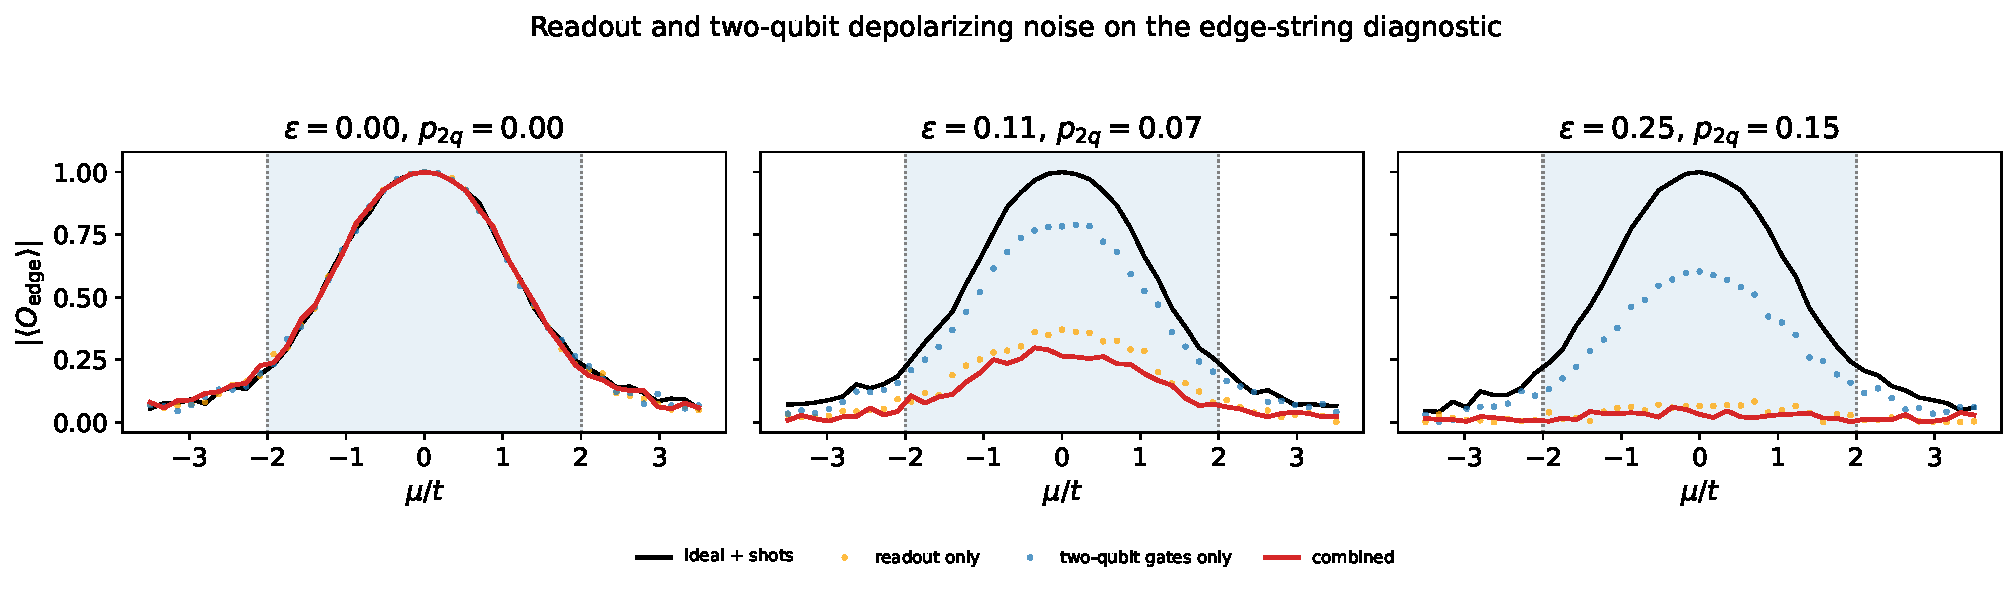
\includegraphics[width=0.95\linewidth]{../plots/block4_week8_noise_sweep.pdf}
  \caption{Readout and two-qubit depolarizing noise applied to the edge-string diagnostic using the same Hamiltonian and edge-string operator as Block 3.}
\end{figure}

\section{Interpretation}

The main effect is loss of contrast. In the topological region $|\mu|<2t$, the ideal edge-string signal is large; readout and depolarizing noise reduce it. In the trivial region, the signal should remain close to zero, but finite shots and noise can create fluctuations around zero. As the noise increases, the separation between the topological and trivial regions becomes less reliable.

The critical regions near $|\mu|=2t$ are naturally the most fragile. Even without noise, the string signal changes rapidly there. Noise therefore does not need to be very large to blur the apparent transition boundary.

This is the first Block 4 diagnostic: it tests whether the observable itself remains readable under controlled noise. The next step is stricter: apply noise during the actual VQE optimization, where the optimizer must search using noisy cost-function evaluations rather than receiving a frozen validated state.

\end{document}
